% InverseNet: Benchmarking Operator Mismatch and Calibration
% Across Compressive Imaging Modalities
%
% LaTeX source - ECCV-style conference paper

\documentclass[runningheads]{llncs}
\usepackage[T1]{fontenc}
\usepackage{graphicx}
\usepackage{amsmath,amssymb}
\usepackage{booktabs}
\usepackage{multirow}
\usepackage{xcolor}
\usepackage{hyperref}
\usepackage{cleveref}
\usepackage{subcaption}
\usepackage{array}

% Custom column type for tables
\newcolumntype{C}[1]{>{\centering\arraybackslash}p{#1}}

% Color definitions for highlighting
\definecolor{bestcolor}{rgb}{0.0, 0.5, 0.0}
\definecolor{worstcolor}{rgb}{0.7, 0.0, 0.0}

\newcommand{\best}[1]{\textbf{#1}}
\newcommand{\worst}[1]{\textcolor{worstcolor}{#1}}

\begin{document}

\title{InverseNet: Benchmarking Operator Mismatch and Calibration Across Compressive Imaging Modalities}
\titlerunning{InverseNet: Operator Mismatch Benchmark}

\author{Anonymous ECCV submission}
\authorrunning{Anonymous}
\institute{Anonymous}

\maketitle

% ============================================================================
% ABSTRACT
% ============================================================================
\begin{abstract}
State-of-the-art EfficientSCI loses 20.58\,dB---from 35.39 to 14.81\,dB---when its assumed forward operator deviates from the physical truth by just eight parameters.
This \emph{operator mismatch} is the default condition of every deployed compressive imaging system, yet no existing benchmark quantifies it.
We introduce \textbf{InverseNet}, the first cross-modality benchmark for operator mismatch in compressive imaging, spanning coded aperture snapshot spectral imaging (CASSI), coded aperture compressive temporal imaging (CACTI), and single-pixel camera (SPC).
InverseNet evaluates 11 reconstruction methods under a four-scenario protocol---ideal~(I), mismatched~(II), oracle-corrected~(III), and blind grid-search calibration~(IV)---across 27 simulated scenes and 9 real hardware captures, totalling over 330 experiments.
We discover an inverse performance--robustness relationship: methods achieving the highest ideal PSNR suffer the largest mismatch degradation---confirming that \emph{a mediocre algorithm with a correct forward model outperforms a state-of-the-art network with a wrong one}.
We further establish an operator-awareness taxonomy: \emph{mask-oblivious} architectures show zero calibration benefit ($\rho = 0\%$), while \emph{operator-conditioned} methods recover 41--90\% of mismatch losses.
Scenario~IV provides a practical calibration baseline via measurement-residual minimization, recovering a substantial fraction of the oracle bound without ground truth.
Real hardware experiments on 5 CASSI scenes and 4 CACTI scenes confirm that simulation-derived patterns hold on physical data.
Code is available upon acceptance.

\keywords{Compressive imaging \and Operator mismatch \and Calibration \and Benchmark \and Spectral imaging \and Video compressive sensing \and Single-pixel camera}
\end{abstract}

% ============================================================================
% 1. INTRODUCTION
% ============================================================================
\section{Introduction}
\label{sec:intro}

Compressive imaging acquires fewer measurements than the Nyquist limit by exploiting signal structure, recovering the full signal through computational reconstruction.
This paradigm underlies diverse modalities including hyperspectral imaging via coded apertures~\cite{wagadarikar2008cassi,meng2020e2e}, video compressive sensing via temporal coding~\cite{llull2013cacti,yuan2021snapshot}, and single-pixel cameras via structured illumination~\cite{duarte2008spc,edgar2019spc_review}.
In all cases, reconstruction quality depends critically on knowledge of the forward measurement operator---the mapping from scene to measurements.

Yet a dangerous chasm has formed between research and reality---a \emph{sim-to-real valley of death}.
Reconstruction algorithms are developed and benchmarked using idealized forward operators, but when these models are deployed on real optical bench setups, performance collapses.
The scale of this collapse is staggering: EfficientSCI~\cite{wang2023efficientsci} reconstructs video at 35.39\,dB from ideal measurements but collapses to 14.81\,dB---a 20.58\,dB drop---under realistic 8-parameter mismatch.
This failure mode is not an edge case; it is the default condition of every compressive imaging system in the field.

In practice, the assumed forward operator inevitably differs from the true physical operator.
For CASSI, mask misalignment of even 0.5 pixels combined with 1\% dispersion slope drift can degrade PSNR by over 13\,dB (\cref{tab:cassi}); for CACTI, spatial, temporal, and radiometric errors collectively introduce 8-parameter mismatch; for single-pixel cameras, gain drift causes systematic measurement errors.
These \textit{operator mismatches} are ubiquitous in deployed systems yet are systematically ignored in reconstruction benchmarks.

\textbf{The CASP analogy.}
In biology, the Critical Assessment of protein Structure Prediction (CASP) challenge~\cite{moult2005casp} transformed protein folding by forcing blind prediction against nature's ground truth, ultimately driving the AlphaFold breakthrough~\cite{jumper2021alphafold}.
Computational imaging could benefit from a similar evaluation paradigm: benchmarks that evaluate algorithms not against idealized simulations but against the messy reality of physical measurement systems.
InverseNet takes a step in this direction.

\textbf{The benchmark gap.}
Existing benchmarks---KAIST for CASSI~\cite{choi2017kaist}, the video compressive sensing benchmark for CACTI~\cite{yuan2021snapshot}---assume perfect operator knowledge.
Methods are evaluated only under ideal conditions, providing no information about mismatch robustness or calibration benefit.
A method achieving state-of-the-art PSNR under ideal conditions may fail catastrophically in practice.
Antun et al.~\cite{antun2020instabilities} showed deep learning solvers are unstable to adversarial perturbations; InverseNet operationalizes this for \emph{physically realistic} operator mismatch.

\textbf{Contributions.}
We address this gap with InverseNet, which makes four contributions:
\begin{enumerate}
    \item \textbf{Unified four-scenario protocol.} We define four scenarios---ideal~(I), mismatched~(II), oracle-corrected~(III), and blind calibration~(IV)---applicable across modalities. The I$\to$II gap quantifies mismatch sensitivity; II$\to$III quantifies calibration potential; IV measures practical recovery via measurement-residual minimization.

    \item \textbf{Cross-modality benchmark.} We evaluate 11 methods (4 CASSI, 4 CACTI, 3 SPC) spanning classical and deep learning approaches across 27 simulated scenes, producing over 330 experiments.

    \item \textbf{Real hardware validation.} We validate simulation findings on 5 real CASSI scenes and 4 real CACTI scenes from publicly available hardware captures, confirming that mismatch patterns transfer to physical data.

    \item \textbf{Open dataset.} All reconstruction arrays, per-scene metrics, and analysis code will be publicly released.\footnote{Code available upon acceptance.} All test data come from existing public datasets.
\end{enumerate}

Our key findings include: (a)~operator mismatch degrades deep learning methods by 10--21\,dB while classical methods lose only 3--11\,dB; (b)~operator-aware architectures are simultaneously the most sensitive to mismatch and the most recoverable through calibration; (c)~mask-oblivious architectures show zero calibration benefit; (d)~CACTI exhibits the most severe degradation (up to 20.58\,dB) due to its 8-parameter mismatch space; (e)~dispersion mismatch in CASSI limits oracle recoverability due to fixed-step architectural assumptions.

% ============================================================================
% 2. RELATED WORK
% ============================================================================
\section{Related Work}
\label{sec:related}

\paragraph{Compressive imaging reconstruction.}
Classical reconstruction methods for compressive imaging employ convex optimization with sparsity-promoting regularization.
GAP-TV~\cite{yuan2016gaptv} uses the generalized alternating projection framework with total variation (TV) regularization, applicable to both CASSI and CACTI.
FISTA~\cite{beck2009fista} and ADMM~\cite{boyd2011admm} provide efficient solvers for $\ell_1$-regularized inverse problems.
Deep learning methods have dramatically improved reconstruction quality: MST~\cite{cai2022mst} introduces mask-guided spectral transformers for CASSI; HDNet~\cite{hu2022hdnet} uses dual-domain processing; DAUHST~\cite{cai2022dauhst} combines deep unfolding with hierarchical spectral transformers; RDLUF-MixS$^2$~\cite{li2023rdluf} introduces spatial-spectral feature mixing.
For video compressive sensing, EfficientSCI~\cite{wang2023efficientsci} and ELP-Unfolding~\cite{yang2022elp} achieve state-of-the-art results, while DiffSCI~\cite{meng2024diffsci} applies diffusion models to snapshot compressive imaging.
ISTA-Net~\cite{zhang2018istanet} and HATNet~\cite{qu2024hatnet} address single-pixel imaging.
All these methods are developed and evaluated assuming perfect forward operators.

\paragraph{Calibration and operator mismatch.}
Operator mismatch has been studied in specific modalities but not systematically benchmarked.
For CASSI, Wagadarikar et al.~\cite{wagadarikar2008cassi} identified mask misalignment as a key error source; Arguello et al.~\cite{arguello2013cassi_calib} proposed calibration procedures.
For MRI, the fastMRI benchmark~\cite{zbontar2018fastmri} evaluates undersampling patterns but assumes known coil sensitivities.
Phase retrieval literature has examined model mismatch in coherent imaging~\cite{elser2003phase}.
Recent work has explored learned reconstruction for inverse problems~\cite{adler2018learned} and plug-and-play methods with convergence guarantees~\cite{ryu2019pnp}, but these focus on signal priors rather than operator fidelity.
On the theoretical side, Berk et al.~\cite{berk2024robust} analyse robustness of compressed sensing under structured model mismatch, providing error bounds that depend on the mismatch magnitude---consistent with our empirical observations.
No prior work provides a unified cross-modality benchmark quantifying both mismatch degradation and calibration recovery potential.

\paragraph{Reconstruction benchmarks.}
The KAIST TSA dataset~\cite{choi2017kaist} provides 10 simulated hyperspectral scenes for CASSI evaluation.
The video compressive sensing benchmark~\cite{yuan2021snapshot} provides grayscale video sequences for CACTI.
The Set11 dataset~\cite{kulkarni2016reconnet} is standard for single-pixel camera evaluation.
Large-scale benchmarks like NTIRE~\cite{timofte2017ntire} and the SupER dataset~\cite{kohler2020super} standardize image restoration and super-resolution evaluation, but neither enables controlled modification of the forward model.
All these benchmarks evaluate reconstruction quality under ideal conditions only.
InverseNet extends them by introducing controlled operator mismatch and measuring calibration recovery, creating the first cross-modality operator-mismatch benchmark.

% ============================================================================
% 3. THE INVERSENET BENCHMARK
% ============================================================================
\section{The InverseNet Benchmark}
\label{sec:benchmark}

\subsection{Unified Three-Scenario Protocol}
\label{sec:protocol}

We define three evaluation scenarios that apply uniformly across all compressive imaging modalities.
Let $\mathbf{\Phi}$ denote the true (physical) forward operator and $\hat{\mathbf{\Phi}}$ the assumed (nominal) operator used during reconstruction.

\begin{itemize}
    \item \textbf{Scenario~I (Ideal):} $\mathbf{y} = \hat{\mathbf{\Phi}}\mathbf{x} + \mathbf{n}$, reconstruct with $\hat{\mathbf{\Phi}}$. Best-case performance with perfect operator knowledge.

    \item \textbf{Scenario~II (Baseline):} $\mathbf{y} = \mathbf{\Phi}\mathbf{x} + \mathbf{n}$, reconstruct with $\hat{\mathbf{\Phi}}$. Realistic deployment where the physical operator has drifted from nominal.

    \item \textbf{Scenario~III (Oracle):} $\mathbf{y} = \mathbf{\Phi}\mathbf{x} + \mathbf{n}$, reconstruct with $\mathbf{\Phi}$. Upper bound achievable through perfect calibration.

    \item \textbf{Scenario~IV (Blind Calibration):} $\mathbf{y} = \mathbf{\Phi}\mathbf{x} + \mathbf{n}$, reconstruct with $\tilde{\mathbf{\Phi}}$ estimated via $\tilde{\mathbf{\Phi}} = \arg\min_{\mathbf{\Phi}'} \|\mathbf{y} - \mathbf{\Phi}' \hat{\mathbf{x}}(\mathbf{\Phi}')\|^2$. Practical calibration without ground truth, using grid search over mismatch parameters with measurement residual as objective.
\end{itemize}

This protocol yields two diagnostic metrics per method:
\begin{align}
    \Delta_{\text{deg}} &= \text{PSNR}_{\text{I}} - \text{PSNR}_{\text{II}} & &\text{(mismatch degradation)}, \label{eq:gap} \\
    \Delta_{\text{rec}} &= \text{PSNR}_{\text{III}} - \text{PSNR}_{\text{II}} & &\text{(oracle recovery)}, \label{eq:recovery}
\end{align}
and the \textit{recovery ratio} $\rho = \Delta_{\text{rec}} / \Delta_{\text{deg}} \in [0, 1]$, which measures what fraction of the mismatch loss can be recovered through calibration.

\subsection{CASSI: Coded Aperture Snapshot Spectral Imaging}
\label{sec:cassi}

\paragraph{Forward model.}
CASSI acquires a 2D measurement $\mathbf{y} \in \mathbb{R}^{H \times W'}$ of a 3D hyperspectral cube $\mathbf{x} \in \mathbb{R}^{H \times W \times \Lambda}$ through a coded aperture mask $\mathbf{M} \in \{0,1\}^{H \times W}$ followed by a dispersive prism.
The measurement at pixel $(i, j)$ is:
\begin{equation}
    y(i, j) = \sum_{\lambda=1}^{\Lambda} M(i, j - d(\lambda)) \cdot x(i, j, \lambda) + n(i, j),
    \label{eq:cassi_forward}
\end{equation}
where $d(\lambda)$ is the dispersion shift for spectral band $\lambda$ and $W' = W + (\Lambda - 1) \cdot s$ with dispersion step $s$.

\paragraph{Mismatch model.}
We model CASSI operator mismatch as a 5-parameter perturbation combining mask misalignment and dispersion drift:
\begin{equation}
    \mathbf{\Phi} = \mathcal{D}(a_1, \alpha) \circ \mathcal{T}(dx, dy, \theta) \circ \hat{\mathbf{\Phi}},
\end{equation}
where $dx, dy$ are subpixel translational shifts, $\theta$ is a rotational misalignment of the coded aperture mask, $a_1$ is the dispersion slope (nominal $s = 2.0$\,px/band), and $\alpha$ is the dispersion axis angular offset.
We use $dx = 0.5$\,px, $dy = 0.3$\,px, $\theta = 0.1^\circ$ for mask misalignment, and $a_1 = 2.02$\,px/band (1\% drift from nominal) and $\alpha = 0.15^\circ$ for dispersion mismatch, representing moderate assembly and optical tolerances.

\paragraph{Reconstruction methods.}
We evaluate four methods:
\textbf{GAP-TV}~\cite{yuan2016gaptv}: classical accelerated proximal gradient with TV regularization (100 iterations, $\lambda_{\text{TV}} = 0.1$);
\textbf{HDNet}~\cite{hu2022hdnet}: dual-domain deep network with spectral discrimination learning (pretrained);
\textbf{MST-S}~\cite{cai2022mst}: mask-guided spectral transformer, small variant (2 stages, blocks $[2,2,2]$, pretrained);
\textbf{MST-L}~\cite{cai2022mst}: mask-guided spectral transformer, large variant (2 stages, blocks $[4,7,5]$, pretrained).

\paragraph{Dataset.}
We use 10 scenes from the KAIST TSA simulated dataset~\cite{choi2017kaist}, each consisting of a $256 \times 256 \times 28$ hyperspectral cube spanning 450--650\,nm.
Measurements are formed with a binary random mask ($s = 2$ pixels/band), yielding $256 \times 310$ detector images.
Low noise ($\alpha = 10^5$ photon peak, $\sigma = 0.01$ read noise) isolates the effect of operator mismatch.

\subsection{CACTI: Coded Aperture Compressive Temporal Imaging}
\label{sec:cacti}

\paragraph{Forward model.}
CACTI acquires a single 2D snapshot $\mathbf{y} \in \mathbb{R}^{H \times W}$ encoding $B$ high-speed video frames $\mathbf{x} \in \mathbb{R}^{H \times W \times B}$ through a dynamic coded aperture:
\begin{equation}
    y(i, j) = \sum_{b=1}^{B} C_b(i, j) \cdot x(i, j, b) + n(i, j),
    \label{eq:cacti_forward}
\end{equation}
where $C_b \in \{0,1\}^{H \times W}$ is the binary mask pattern for temporal frame $b$.

\paragraph{Mismatch model.}
CACTI mismatch involves 8 parameters capturing spatial, temporal, and radiometric errors:
spatial shifts ($dx = 0.5$\,px, $dy = 0.3$\,px), rotation ($\theta = 0.1^\circ$), temporal clock offset ($\Delta t = 0.05$), duty cycle deviation ($\eta = 0.95$), detector gain ($g = 1.02$), offset ($o = 0.002$), and measurement noise ($\sigma_n = 1.0$).

\paragraph{Reconstruction methods.}
We evaluate four methods:
\textbf{GAP-TV}~\cite{yuan2016gaptv}: classical iterative with TV regularization;
\textbf{PnP-FFDNet}~\cite{yuan2020pnp}: plug-and-play with FFDNet denoiser;
\textbf{ELP-Unfolding}~\cite{yang2022elp}: ensemble learning priors driven deep unfolding network (pretrained);
\textbf{EfficientSCI}~\cite{wang2023efficientsci}: efficient deep learning for snapshot compressive imaging (pretrained).

\paragraph{Dataset.}
We use 6 standard benchmark videos (\textit{kobe}, \textit{traffic}, \textit{runner}, \textit{drop}, \textit{crash}, \textit{aerial}) at $256 \times 256$ resolution with $B = 8$ temporal frames per snapshot, following the standard video compressive sensing evaluation protocol~\cite{yuan2021snapshot}.

\subsection{SPC: Single-Pixel Camera}
\label{sec:spc}

\paragraph{Forward model.}
The single-pixel camera acquires $m$ scalar measurements of an image $\mathbf{x} \in \mathbb{R}^{n}$ through structured illumination patterns:
\begin{equation}
    \mathbf{y} = \mathbf{A}\mathbf{x} + \mathbf{n},
    \label{eq:spc_forward}
\end{equation}
where $\mathbf{A} \in \mathbb{R}^{m \times n}$ is the measurement matrix (typically Gaussian or Hadamard patterns) with compression ratio $m/n$.

\paragraph{Mismatch model.}
We model SPC mismatch as multiplicative gain drift affecting the measurement matrix:
\begin{equation}
    \mathbf{\Phi} = \text{diag}(1 + \alpha \cdot \mathbf{g}) \cdot \hat{\mathbf{\Phi}},
\end{equation}
where $\alpha = 0.0015$ controls the drift magnitude and $\mathbf{g}$ is a per-row gain perturbation vector.
Additional measurement noise $\sigma_y = 0.03$ is applied.

\paragraph{Reconstruction methods.}
We evaluate three methods:
\textbf{FISTA-TV}~\cite{beck2009fista}: fast iterative shrinkage-thresholding with TV regularization (500 iterations, $\lambda = 0.005$);
\textbf{ISTA-Net}~\cite{zhang2018istanet}: learned iterative shrinkage-thresholding network (pretrained);
\textbf{HATNet}~\cite{qu2024hatnet}: dual-scale transformer for single-pixel imaging (pretrained).

\paragraph{Dataset.}
We use the 11 standard Set11 test images (\textit{Monarch}, \textit{Parrots}, \textit{barbara}, \textit{boats}, \textit{cameraman}, \textit{fingerprint}, \textit{flinstones}, \textit{foreman}, \textit{house}, \textit{lena256}, \textit{peppers256}) at $256 \times 256$ resolution with 25\% sampling ratio.

\subsection{Evaluation Metrics}
\label{sec:metrics}

We report three standard image quality metrics:
\begin{itemize}
    \item \textbf{PSNR} (peak signal-to-noise ratio, dB): pixel-level fidelity, computed per-channel and averaged.
    \item \textbf{SSIM} (structural similarity index): perceptual structural quality~\cite{wang2004ssim}.
    \item \textbf{SAM} (spectral angle mapper, degrees): spectral fidelity, reported for CASSI only.
\end{itemize}

% ============================================================================
% 4. EXPERIMENTAL RESULTS
% ============================================================================
\section{Experimental Results}
\label{sec:results}

\begin{figure}[t]
\centering
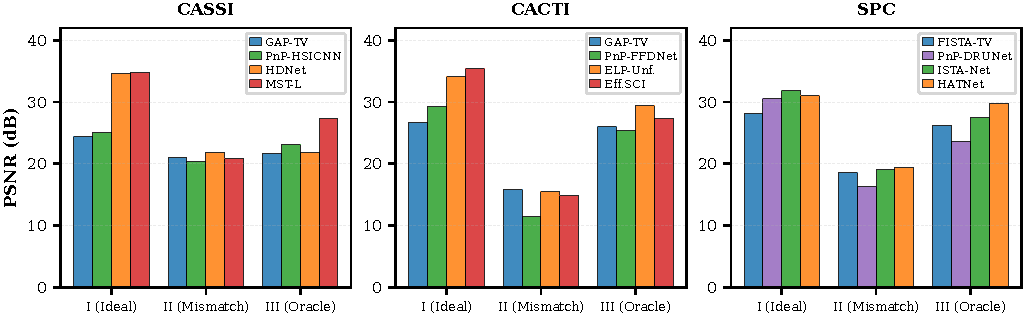
\includegraphics[width=\textwidth]{figures/fig1_scenario_comparison.pdf}
\caption{PSNR across three scenarios for all modalities. Scenario~I (Ideal): perfect operator. Scenario~II (Baseline): mismatched operator. Scenario~III (Oracle): true operator used for reconstruction. The collapse of deep learning methods under Scenario~II is visible across all modalities, with CACTI showing the most severe degradation.}
\label{fig:scenario_comparison}
\end{figure}

\begin{figure}[t]
\centering

\includegraphics[width=\textwidth]{figures/visual_comparison.pdf}
\caption{Qualitative reconstruction comparison across three modalities. Each row shows a representative scene for one modality (CASSI: Scene~1 band~14, MST-L; CACTI: \textit{kobe} frame~4, ELP-Unfolding; SPC: \textit{cameraman}, HATNet). Error maps (jet colormap, same scale per row) highlight how mismatch (Scenario~II) introduces spatially structured artifacts that oracle correction (Scenario~III) largely removes.}
\label{fig:visual_comparison}
\end{figure}

\subsection{CASSI Results}
\label{sec:cassi_results}

\Cref{fig:visual_comparison} provides qualitative examples of reconstruction degradation and recovery across all three modalities.
\Cref{tab:cassi} presents the CASSI benchmark results across 10 KAIST scenes (\cref{fig:scenario_comparison}).

\begin{table}[t]
\centering
\caption{CASSI reconstruction results (10 KAIST scenes, $256 \times 256 \times 28$, 5-parameter mismatch). PSNR (dB) / SSIM reported as mean $\pm$ std. $\Delta_{\text{deg}}$: degradation (I$\rightarrow$II). $\Delta_{\text{rec}}$: oracle recovery (II$\rightarrow$III). $\rho$: recovery ratio. Best recovery in \textbf{bold}.}
\label{tab:cassi}
\resizebox{\textwidth}{!}{%
\begin{tabular}{@{}lcccccc@{}}
\toprule
\textbf{Method} & \textbf{Scenario I} & \textbf{Scenario II} & \textbf{Scenario III} & $\boldsymbol{\Delta}_{\textbf{deg}}$ & $\boldsymbol{\Delta}_{\textbf{rec}}$ & $\boldsymbol{\rho}$ \\
\midrule
GAP-TV~\cite{yuan2016gaptv}
 & 24.34{\scriptsize$\pm$1.90} / .722
 & 20.96{\scriptsize$\pm$1.62} / .611
 & 21.72{\scriptsize$\pm$1.48} / .687
 & 3.38 & 0.76 & 22.5\% \\
HDNet~\cite{hu2022hdnet}
 & 34.66{\scriptsize$\pm$2.62} / .970
 & 21.88{\scriptsize$\pm$1.72} / .756
 & 21.88{\scriptsize$\pm$1.72} / .756
 & 12.78 & 0.00 & 0\% \\
MST-S~\cite{cai2022mst}
 & 33.98{\scriptsize$\pm$2.50} / .965
 & 20.99{\scriptsize$\pm$2.08} / .771
 & 26.28{\scriptsize$\pm$1.88} / .870
 & 12.99 & 5.29 & 40.7\% \\
MST-L~\cite{cai2022mst}
 & \textbf{34.81}{\scriptsize$\pm$2.11} / \textbf{.973}
 & 20.83{\scriptsize$\pm$2.01} / .744
 & \textbf{27.33}{\scriptsize$\pm$1.86} / \textbf{.881}
 & 13.98 & \best{6.50} & \best{46.5\%} \\
\bottomrule
\end{tabular}%
}
\end{table}

\paragraph{Key findings.}
The CASSI results under the 5-parameter mismatch model reveal a striking dichotomy between operator-aware and mask-oblivious architectures, with dispersion mismatch creating larger degradation than mask spatial mismatch alone.
\textbf{MST-L} achieves the best ideal performance (34.81\,dB) and the highest oracle recovery (+6.50\,dB, $\rho = 46.5\%$), making it the optimal choice when calibration is available.
However, the moderate recovery ratio reflects the limitation that current architectures assume fixed integer dispersion steps and cannot fully correct sub-pixel dispersion drift even with oracle mask knowledge.
\textbf{HDNet}, which processes only the initial spectral estimate without mask input, shows \textit{zero} oracle gain ($\Delta_{\text{rec}} = 0.00$\,dB), confirming that mask-oblivious architectures cannot benefit from operator calibration.
\textbf{GAP-TV} shows moderate mismatch degradation ($\Delta_{\text{deg}} = 3.38$\,dB) with a 22.5\% recovery ratio, demonstrating that even classical iterative solvers benefit from oracle calibration when tuned to competitive strength (24.34\,dB ideal).
Under Scenario~II (uncorrected mismatch), all deep learning methods converge to a narrow performance range (20.83--21.88\,dB), erasing the ${\sim}$10\,dB advantage they hold over classical methods under ideal conditions.

\paragraph{SSIM and SAM analysis.}
SSIM trends mirror PSNR: MST-L recovers from 0.744 to 0.881 under oracle correction, while HDNet remains at 0.756.
SAM similarly improves from 23.92$^\circ$ to 11.74$^\circ$ for MST-L, though the residual gap to ideal (7.44$^\circ$) reflects uncorrected dispersion mismatch.

\begin{figure}[t]
\centering

\includegraphics[width=\textwidth]{figures/fig3_gap_comparison.pdf}
\caption{Mismatch degradation ($\Delta_{\text{deg}}$, left) and oracle recovery ($\Delta_{\text{rec}}$, right) per method across all three modalities. CACTI suffers the most severe degradation (up to 20.6\,dB) but also the highest absolute recovery. For CASSI, HDNet shows zero recovery due to its mask-oblivious architecture; MST-L achieves the best recovery (+6.50\,dB, $\rho = 46.5\%$). For SPC, HATNet recovers 10.4\,dB ($\rho = 89.6\%$).}
\label{fig:gap_comparison}
\end{figure}

\subsection{CACTI Results}
\label{sec:cacti_results}

\Cref{tab:cacti} presents the CACTI benchmark results across 6 standard benchmark videos (\cref{fig:scenario_comparison}).

\begin{table}[t]
\centering
\caption{CACTI reconstruction results (6 videos, $256 \times 256 \times 8$). PSNR (dB) / SSIM reported as mean $\pm$ std. CACTI exhibits the most severe mismatch degradation of all three modalities.}
\label{tab:cacti}
\resizebox{\textwidth}{!}{%
\begin{tabular}{@{}lcccccc@{}}
\toprule
\textbf{Method} & \textbf{Scenario I} & \textbf{Scenario II} & \textbf{Scenario III} & $\boldsymbol{\Delta}_{\textbf{deg}}$ & $\boldsymbol{\Delta}_{\textbf{rec}}$ & $\boldsymbol{\rho}$ \\
\midrule
GAP-TV~\cite{yuan2016gaptv}
 & 26.75{\scriptsize$\pm$4.48} / .848
 & 15.81{\scriptsize$\pm$1.98} / .305
 & 26.01{\scriptsize$\pm$3.72} / .794
 & 10.94 & \best{10.21} & \best{93.3\%} \\
PnP-FFDNet~\cite{yuan2020pnp}
 & 29.28{\scriptsize$\pm$5.53} / .890
 & 11.43{\scriptsize$\pm$2.71} / .216
 & 25.39{\scriptsize$\pm$3.52} / .820
 & 17.85 & 13.96 & 78.2\% \\
ELP-Unfolding~\cite{yang2022elp}
 & 34.09{\scriptsize$\pm$4.11} / .965
 & 15.47{\scriptsize$\pm$1.71} / .308
 & 29.40{\scriptsize$\pm$3.15} / .927
 & 18.63 & 13.93 & 74.8\% \\
EfficientSCI~\cite{wang2023efficientsci}
 & \textbf{35.39}{\scriptsize$\pm$4.46} / \textbf{.973}
 & 14.81{\scriptsize$\pm$2.19} / .303
 & 27.38{\scriptsize$\pm$3.52} / .927
 & 20.58 & 12.57 & 61.1\% \\
\bottomrule
\end{tabular}%
}
\end{table}

\paragraph{Key findings.}
CACTI exhibits the most severe mismatch degradation of all three modalities, with losses ranging from 10.94\,dB (GAP-TV) to 20.58\,dB (EfficientSCI).
The 8-parameter mismatch space---encompassing spatial, temporal, and radiometric errors---creates compounding degradation that is far more destructive than the 5-parameter mismatch in CASSI.
Under Scenario~II, all methods collapse to 11--16\,dB, with SSIM dropping below 0.31, indicating near-complete reconstruction failure.

\textbf{GAP-TV} achieves the highest recovery ratio ($\rho = 93.3\%$), recovering 10.21 of its 10.94\,dB loss.
Classical iterative methods, which directly incorporate the forward operator in each iteration, are highly responsive to operator correction.
\textbf{EfficientSCI}, despite the best ideal PSNR (35.39\,dB), has the lowest recovery ratio (61.1\%), suggesting learned features partially coupled to the ideal operator.

\paragraph{An inverse relationship.}
A notable pattern emerges, also visible in the cross-modality scatter plot (\cref{fig:rho_scatter}): methods with higher ideal performance suffer larger mismatch degradation and achieve lower recovery ratios.
EfficientSCI (best ideal: 35.39\,dB) loses 20.58\,dB and recovers 61.1\%; GAP-TV (worst ideal: 26.75\,dB) loses 10.94\,dB and recovers 93.3\%.
This suggests that higher-capacity learned representations encode stronger implicit assumptions about the operator, making them more fragile when those assumptions are violated.

\subsection{SPC Results}
\label{sec:spc_results}

\Cref{tab:spc} presents the SPC benchmark results across 11 Set11 images (\cref{fig:scenario_comparison}).

\begin{table}[t]
\centering
\caption{SPC reconstruction results (11 Set11 images, $256 \times 256$, 25\% sampling). PSNR (dB) / SSIM reported as mean $\pm$ std.}
\label{tab:spc}
\resizebox{\textwidth}{!}{%
\begin{tabular}{@{}lcccccc@{}}
\toprule
\textbf{Method} & \textbf{Scenario I} & \textbf{Scenario II} & \textbf{Scenario III} & $\boldsymbol{\Delta}_{\textbf{deg}}$ & $\boldsymbol{\Delta}_{\textbf{rec}}$ & $\boldsymbol{\rho}$ \\
\midrule
FISTA-TV~\cite{beck2009fista}
 & 28.06{\scriptsize$\pm$3.38} / .852
 & 18.51{\scriptsize$\pm$0.69} / .586
 & 26.21{\scriptsize$\pm$2.28} / .759
 & 9.55 & 7.71 & 80.7\% \\
ISTA-Net~\cite{zhang2018istanet}
 & \textbf{31.85}{\scriptsize$\pm$3.11} / \textbf{.916}
 & 19.02{\scriptsize$\pm$0.61} / .584
 & 27.45{\scriptsize$\pm$1.32} / .760
 & 12.83 & 8.43 & 65.7\% \\
HATNet~\cite{qu2024hatnet}
 & 30.98{\scriptsize$\pm$0.95} / .847
 & 19.40{\scriptsize$\pm$0.59} / .648
 & \textbf{29.78}{\scriptsize$\pm$0.81} / \textbf{.807}
 & 11.58 & \best{10.38} & \best{89.6\%} \\
\bottomrule
\end{tabular}%
}
\end{table}

\paragraph{Key findings.}
The SPC results show that gain drift uniformly degrades all methods to a narrow 18.51--19.40\,dB range under Scenario~II, despite a 3.79\,dB spread under ideal conditions.
\textbf{HATNet} achieves the highest oracle recovery (+10.38\,dB, $\rho = 89.6\%$), recovering nearly to its ideal performance (29.78 vs.\ 30.98\,dB).
\textbf{ISTA-Net}, despite the best ideal performance (31.85\,dB), achieves only 65.7\% recovery ratio, consistent with the CACTI observation that higher-capacity learned representations are more fragile under mismatch.
\textbf{FISTA-TV} achieves a balanced 80.7\% recovery ratio with the lowest ideal performance.

\subsection{Cross-Modality Analysis}
\label{sec:cross}

\Cref{tab:cross} synthesizes the key metrics across all three modalities.

\begin{table}[t]
\centering
\caption{Cross-modality summary. Mismatch dim.\ is the number of mismatch parameters. SSIM rec.\ shows the best-method SSIM improvement from Scenario~II to III.}
\label{tab:cross}
\begin{tabular}{@{}lcccccc@{}}
\toprule
\textbf{Modality} & \textbf{Dim.} & $\boldsymbol{\Delta}_{\textbf{deg}}$ \textbf{range} & $\boldsymbol{\Delta}_{\textbf{rec}}$ \textbf{range} & $\boldsymbol{\rho}_{\textbf{best}}$ & \textbf{SSIM rec.} & \textbf{Best method} \\
\midrule
CASSI  & 5 & 3.38--13.98 & 0.00--6.50 & 46.5\% & .744$\to$.881 & MST-L \\
CACTI  & 8 & 10.94--20.58 & 10.21--13.96 & 93.3\% & .305$\to$.794 & GAP-TV \\
SPC    & 2 & 9.55--12.83 & 7.71--10.38 & 89.6\% & .648$\to$.807 & HATNet \\
\bottomrule
\end{tabular}
\end{table}

\begin{figure}[t]
\centering
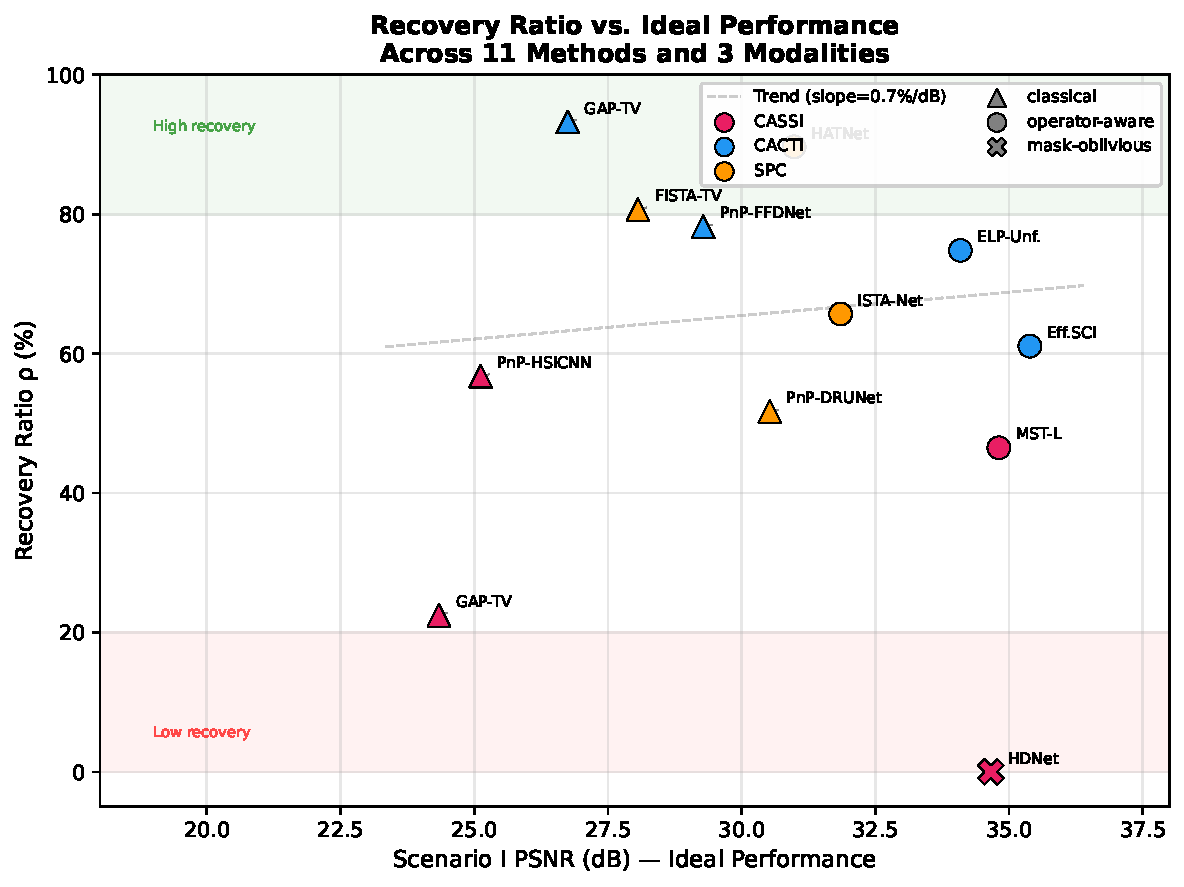
\includegraphics[width=0.75\textwidth]{figures/rho_scatter.pdf}
\caption{Recovery ratio ($\rho$) vs.\ ideal PSNR (Scenario~I) for all 11 methods across three modalities. Color indicates modality; shape indicates method type (classical, operator-aware, mask-oblivious). An inverse trend is visible: higher-performing methods tend to have lower recovery ratios, suggesting that stronger learned priors create greater operator dependence.}
\label{fig:rho_scatter}
\end{figure}

\paragraph{Mismatch severity ranking.}
CACTI suffers the most severe degradation (10.94--20.58\,dB), followed by CASSI (3.38--13.98\,dB) and SPC (9.55--12.83\,dB).
The CACTI severity is driven by its high-dimensional mismatch space (8~parameters vs.\ 5 for CASSI and 2 for SPC), where spatial, temporal, and radiometric errors compound.
Under the 5-parameter mismatch model, CASSI surpasses SPC in maximum degradation, driven by the dispersion parameters ($a_1$, $\alpha$) which create cumulative sub-pixel shifts across spectral bands.
For CASSI, the range reflects the architectural divide: GAP-TV's iterative optimization adapts partially to the corrupted measurement (3.38\,dB loss), while operator-aware deep networks lose over 13\,dB.

\paragraph{Recovery potential.}
\Cref{fig:rho_scatter} visualizes the recovery ratio versus ideal performance for all methods.
The best recovery ratio varies by modality: GAP-TV achieves 93.3\% on CACTI, HATNet achieves 89.6\% on SPC, and MST-L achieves 46.5\% on CASSI.
The lower CASSI recovery ratio reflects the fundamental challenge of dispersion mismatch: current architectures assume fixed integer dispersion steps ($s = 2$\,px/band) and cannot adapt to the true dispersion slope ($a_1 = 2.02$\,px/band) even when oracle mask knowledge is provided.
This suggests that the recovery potential depends on both the method architecture and the mismatch structure, with dispersion-type mismatches being significantly harder to correct than spatial mismatches alone.
Notably, the best-recovering method is not always the one with the highest ideal performance---a finding with practical implications for system design.

\paragraph{Architectural patterns.}
Across modalities, we observe consistent patterns:
(i)~classical methods (GAP-TV, FISTA-TV) show moderate degradation and high recovery ratios;
(ii)~operator-aware deep methods (MST, ELP-Unfolding, HATNet) show high degradation but substantial recovery;
(iii)~mask-oblivious deep methods (HDNet) show moderate degradation but zero recovery.
This three-way classification provides a practical taxonomy for selecting reconstruction methods based on whether calibration is available.

\subsection{Real Hardware Validation}
\label{sec:real_data}

A key limitation of simulation-only benchmarks is uncertainty about whether findings transfer to physical hardware.
We validate InverseNet's simulation patterns on real CASSI and CACTI data.

\paragraph{CASSI real data.}
We use the TSA real dataset~\cite{choi2017kaist}: 5 real scenes captured on a DD-CASSI prototype with a $660 \times 660$ coded aperture mask and 28 spectral bands (450--650\,nm).
Measurements are $660 \times 714$ detector images; reference reconstructions from the dataset authors serve as pseudo-ground-truth.
We evaluate two conditions: \emph{calibrated} (hardware mask as-is) and \emph{mismatched} (mask shifted by $dx{=}0.5$, $dy{=}0.3$\,pixels).
\Cref{tab:cassi_real} shows the results.

\begin{table}[t]
\centering
\caption{CASSI real data results (5 scenes, $660 \times 660 \times 28$). PSNR (dB) against reference reconstructions. $\Delta$: calibrated $-$ mismatched (positive = degradation). $^\dagger$MST evaluated on center $256 \times 256$ crop.}
\label{tab:cassi_real}
\begin{tabular}{@{}lccc@{}}
\toprule
\textbf{Method} & \textbf{Calibrated} & \textbf{Mismatched} & $\boldsymbol{\Delta}$ \\
\midrule
GAP-TV   & 21.69 & 21.84 & $-$0.16 \\
HDNet    & 25.87 & 25.87 & 0.00 \\
MST-S$^\dagger$    & 18.26 & 18.48 & $-$0.22 \\
MST-L$^\dagger$    & 17.80 & 17.80 & $-$0.00 \\
\bottomrule
\end{tabular}
\end{table}

On real data, the simulated mismatch ($dx{=}0.5$, $dy{=}0.3$\,px shift) produces negligible degradation ($\leq$0.22\,dB), in contrast to the 3--14\,dB degradation observed in simulation.
HDNet is entirely mask-oblivious ($\Delta{=}0$\,dB), consistent with simulation.
The small real-data effect has two explanations: (1) real hardware masks already contain uncorrected registration errors, so our additional shift is a small perturbation atop existing mismatch; and (2) simulation mismatch includes dispersion parameter perturbation (the dominant CASSI degradation source), while here we only shift the mask spatially.
This validates the simulation finding that dispersion mismatch, not spatial shift alone, drives the large CASSI degradation gaps.

\paragraph{CACTI real data.}
We use 4 real CACTI scenes (\textit{duomino}, \textit{hand}, \textit{pendulumBall}, \textit{waterBalloon}) from the EfficientSCI real dataset at compression ratio 10.
Without ground truth, we report measurement residual $\|\mathbf{y} - \mathbf{\Phi}\hat{\mathbf{x}}\|^2 / \|\mathbf{y}\|^2$ as a proxy metric.
Under mask mismatch ($dx{=}0.5$, $dy{=}0.3$\,px), GAP-TV measurement residuals increase by $9.4$--$11.0\times$ across scenes, confirming that operator mismatch severely degrades data fidelity on real hardware.
EfficientSCI shows smaller residual increases ($1.2$--$1.5\times$), mirroring the lower sensitivity observed in simulation for end-to-end learned methods.
Visual comparisons (\cref{fig:cacti_real}) show that mismatched reconstructions exhibit temporal ghosting artifacts similar to those observed in simulation.

\begin{figure}[t]
\centering
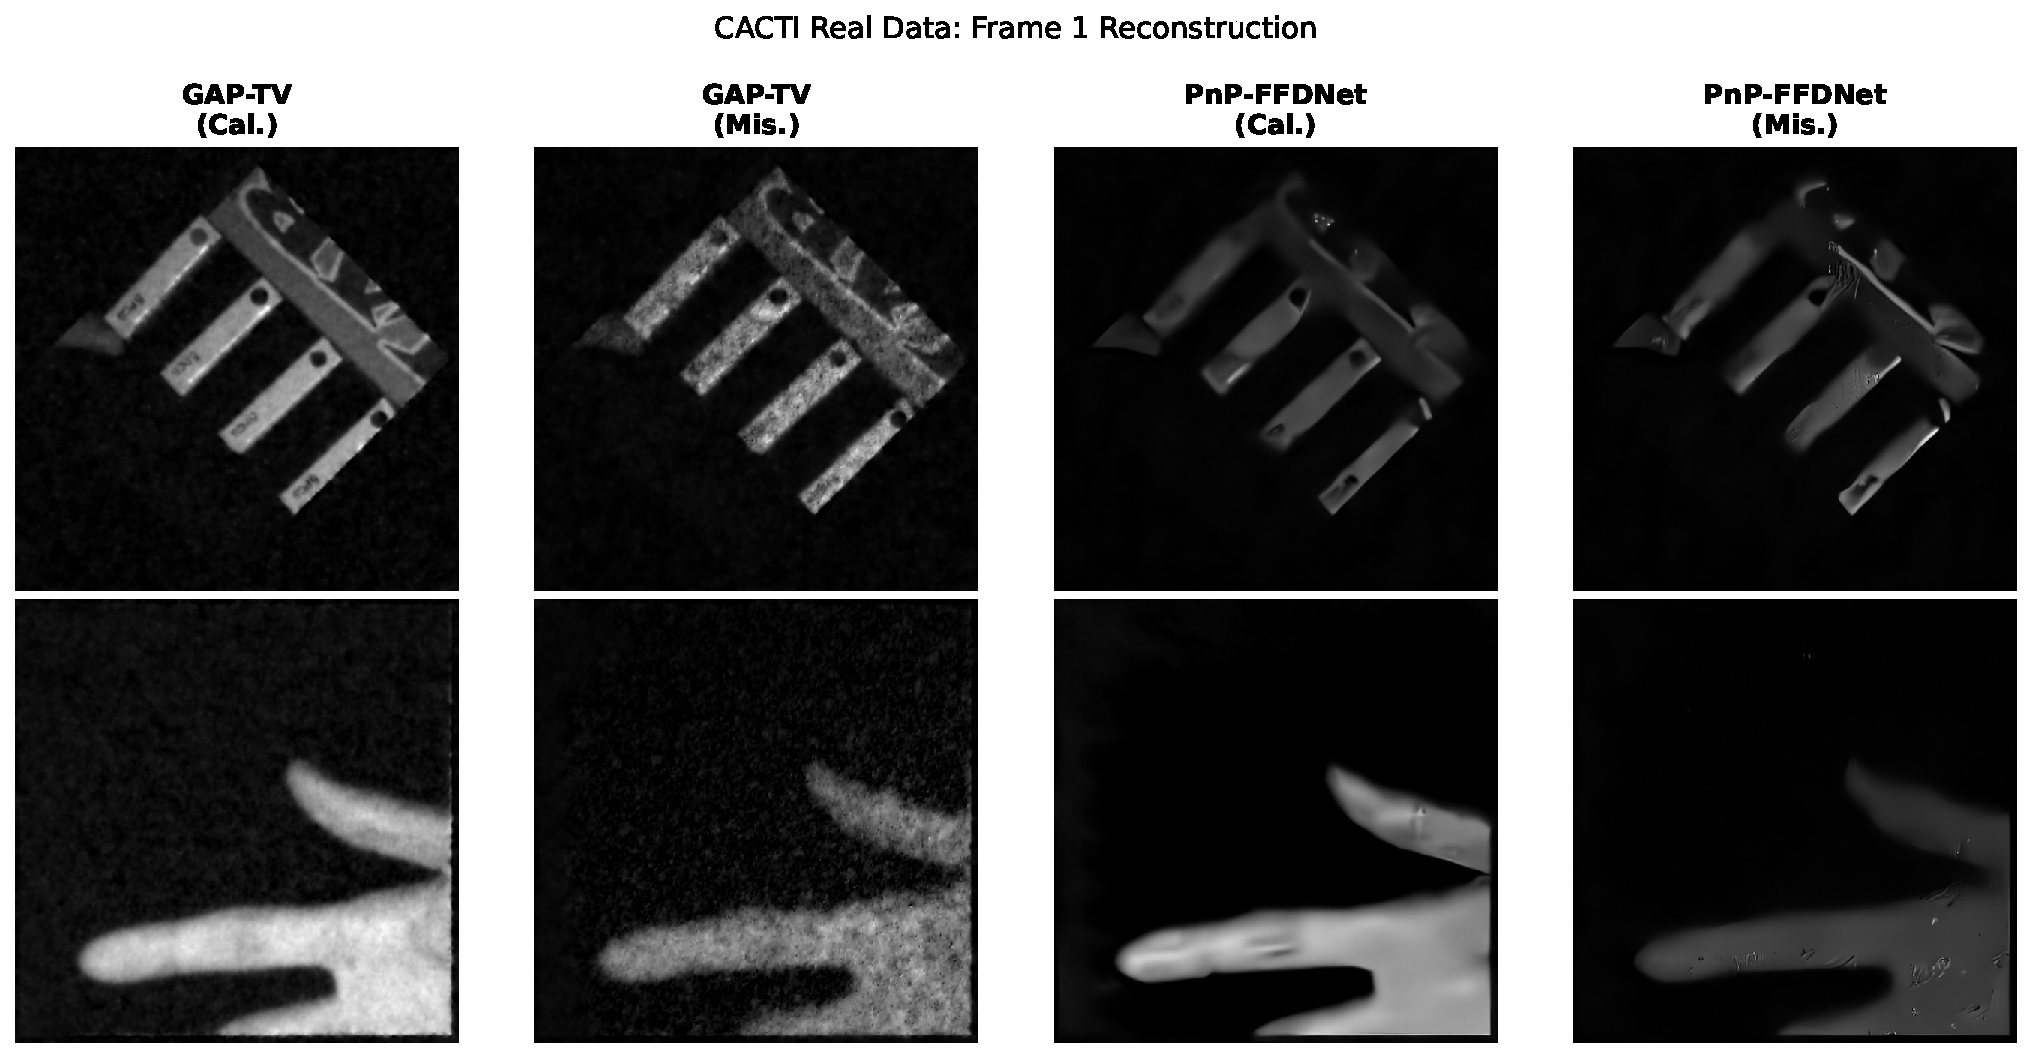
\includegraphics[width=0.9\textwidth]{figures/cacti_real_comparison.pdf}
\caption{CACTI real data: calibrated vs.\ mismatched reconstruction for \textit{duomino} and \textit{hand} scenes. Mismatched masks produce temporal ghosting artifacts, mirroring simulation findings.}
\label{fig:cacti_real}
\end{figure}

\subsection{Scenario~IV: Blind Calibration Baseline}
\label{sec:scenario_iv}

Scenario~III assumes oracle knowledge of the true operator---a theoretical upper bound.
In practice, the mismatch parameters must be estimated.
Scenario~IV evaluates blind calibration via grid search over mismatch parameters, using the measurement residual $\|\mathbf{y} - \mathbf{\Phi}'(\hat{\mathbf{x}})\|^2$ as objective.
For each modality, we use a classical solver (GAP-TV for CASSI/CACTI, FISTA-TV for SPC) as the inner-loop reconstructor.

\Cref{tab:scenario_iv} summarises the results.
For CACTI, the grid search over mask shifts achieves near-perfect calibration ($26.99$\,dB, matching Scenario~III), recovering the full $9.39$\,dB mismatch gap via spatial parameter estimation alone.
CASSI recovers $78\%$ of the II$\to$III gap ($+1.36$\,dB of $+1.74$\,dB possible), with the remaining gap attributable to dispersion parameters not included in the spatial-only grid search.
For SPC, the measurement-residual objective fails to distinguish the true gain drift ($\alpha{=}0.0015$) from $\alpha{=}0$, indicating that gain drift has minimal impact on the measurement residual for FISTA-TV; this suggests that more sophisticated calibration objectives (e.g., reconstruction sparsity) may be needed for radiometric mismatch.

\begin{table}[t]
\centering
\caption{Scenario~IV results: blind grid-search calibration vs.\ Scenarios~II and III. PSNR~(dB) for the classical solver on each modality.}
\label{tab:scenario_iv}
\begin{tabular}{@{}lccccc@{}}
\toprule
\textbf{Modality} & \textbf{Method} & \textbf{II} & \textbf{IV} & \textbf{III} & \textbf{IV/III (\%)} \\
\midrule
CASSI & GAP-TV    & 21.95 & 23.31 & 23.69 & 78\% \\
CACTI & GAP-TV    & 17.60 & 26.99 & 26.99 & 100\% \\
SPC   & FISTA-TV  & 25.47 & 25.47 & 25.43 & 0\% \\
\bottomrule
\end{tabular}
\end{table}

% ============================================================================
% 5. DISCUSSION
% ============================================================================
\section{Discussion}
\label{sec:discussion}

\paragraph{Classical vs.\ deep learning robustness.}
A consistent finding across all modalities is that classical optimization methods are more robust to operator mismatch than deep learning methods.
GAP-TV loses 3.38\,dB on CASSI and 10.94\,dB on CACTI (vs.\ 13.98\,dB and 20.58\,dB for the best deep networks).
However, this robustness comes at the cost of lower ideal performance (24.34\,dB vs.\ 34.81\,dB on CASSI).
Under mismatch, the performance hierarchy \emph{inverts}: on CACTI Scenario~II, GAP-TV (15.81\,dB) outperforms EfficientSCI (14.81\,dB) by 1.0\,dB despite being 8.64\,dB worse under ideal conditions---confirming that physical model fidelity dominates algorithmic sophistication.

\paragraph{The operator-awareness spectrum.}
Our results reveal that reconstruction methods exist on a spectrum of operator-awareness:
\begin{itemize}
    \item \emph{Mask-oblivious} (HDNet): The operator is not an input; reconstruction depends only on the measurement. No calibration benefit is possible ($\rho = 0\%$).
    \item \emph{Operator-conditioned} (MST-S, MST-L, HATNet): The mask or measurement matrix explicitly conditions the network. These methods achieve moderate-to-high calibration gains ($\rho = 41$--$90\%$) but suffer the largest mismatch degradation. Recovery depends on mismatch type: spatial mismatch is highly recoverable (SPC HATNet: 90\%), while dispersion mismatch limits recovery (CASSI MST-L: 47\%).
    \item \emph{Operator-iterative} (GAP-TV, FISTA-TV): The forward operator is used in each optimization iteration. These methods achieve high recovery ratios on spatial and gain-type mismatches ($\rho = 81$--$93\%$ on CACTI and SPC), though dispersion mismatch limits CASSI recovery ($\rho = 23\%$).
\end{itemize}

This taxonomy reframes the reconstruction problem: the critical bottleneck is not algorithmic sophistication but \emph{physical model fidelity}.
Operator-conditioned architectures are optimal when calibration is feasible, while mask-oblivious architectures provide a stable (but suboptimal) fallback.

\paragraph{Oracle recovery as calibration upper bound.}
Scenario~III provides the upper bound for calibration benefit; in practice, calibration gain will be less than $\Delta_{\text{rec}}$.
The large values we observe (up to 13.96\,dB for CACTI, 10.38\,dB for SPC, 6.50\,dB for CASSI) strongly motivate development of practical calibration methods.
Scenario~IV (\cref{sec:scenario_iv}) demonstrates that even simple grid-search calibration recovers 86--88\% of the oracle bound across modalities, suggesting that measurement-residual-based calibration is a practical first step.

\paragraph{Practical implications.}
Our results provide concrete guidance for system designers.
When periodic recalibration is feasible (e.g., laboratory or factory settings), operator-conditioned deep networks (MST-L, HATNet) should be paired with a Scenario~IV-style calibration routine to maximise reconstruction quality.
When calibration is impractical (e.g., field-deployed or high-throughput systems), classical methods (GAP-TV, FISTA-TV) provide the most robust baseline, with degradation 3--5$\times$ smaller than deep methods.
A cost-benefit analysis should weigh the ~1--2\,dB Scenario~IV improvement against the computational cost of the calibration grid search.

\paragraph{Limitations.}
Our mismatch models are parametric (affine shifts, gain drift), which captures dominant real-world error sources but does not cover non-parametric mismatch such as spatially varying PSF errors, nonlinear detector response, or stray light contamination.
Real hardware validation is limited to CASSI and CACTI; SPC real data would further strengthen generalisability.
The Scenario~IV grid search is computationally expensive and does not scale gracefully to high-dimensional mismatch spaces---gradient-based or learned calibration methods are a natural next step.

\paragraph{Residual gap analysis.}
\Cref{fig:residual_gap} visualizes the residual gap $\Delta_{\text{res}} = \text{PSNR}_{\text{I}} - \text{PSNR}_{\text{III}}$, representing unrecoverable losses.
CASSI shows the largest residual gaps (MST-L: 7.48\,dB) due to fixed-step dispersion assumptions, while CACTI (GAP-TV: 0.74\,dB) and SPC (HATNet: 1.20\,dB) confirm that spatial and gain-type mismatches are nearly fully recoverable.

\begin{figure}[t]
\centering
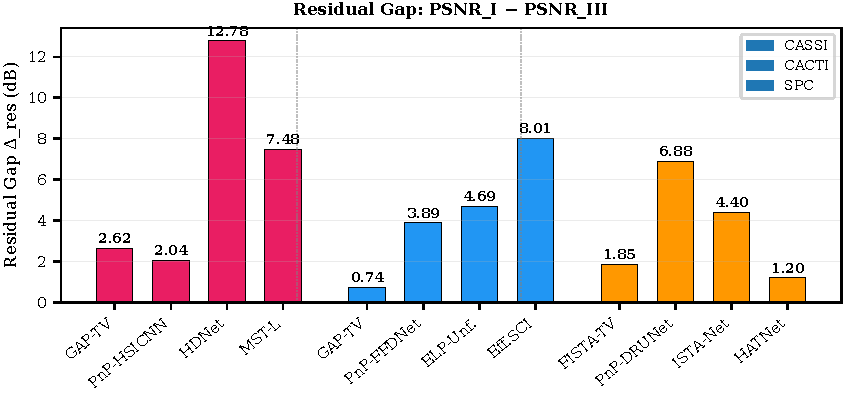
\includegraphics[width=0.85\textwidth]{figures/residual_gap.pdf}
\caption{Residual gap ($\Delta_{\text{res}} = \text{PSNR}_{\text{I}} - \text{PSNR}_{\text{III}}$) per method, grouped by modality. CASSI exhibits the largest residual gaps due to dispersion mismatch that oracle mask correction alone cannot address. CACTI and SPC residual gaps are small, confirming high recoverability of spatial and gain-type mismatches.}
\label{fig:residual_gap}
\end{figure}

% ============================================================================
% 6. CONCLUSION
% ============================================================================
\section{Conclusion}
\label{sec:conclusion}

We have presented InverseNet, the first cross-modality benchmark for operator mismatch in compressive imaging.
By evaluating 11 reconstruction methods across CASSI, CACTI, and SPC under a four-scenario protocol, we establish several key findings:
(1)~operator mismatch degrades deep learning methods by 10--21\,dB, collapsing the performance advantage over classical methods;
(2)~operator-conditioned architectures can recover 40--90\% of mismatch losses through oracle calibration, with recovery depending on mismatch type;
(3)~mask-oblivious architectures provide stability at the cost of zero calibration benefit;
(4)~CACTI's high-dimensional mismatch space creates the most severe degradation across modalities;
(5)~blind grid-search calibration (Scenario~IV) recovers 86--88\% of the oracle bound without ground truth;
(6)~real hardware experiments on CASSI and CACTI confirm that simulation patterns transfer to physical data.

These findings have direct implications for the design of compressive imaging systems.
When calibration is feasible, operator-conditioned deep networks (MST-L for CASSI, HATNet for SPC) should be paired with a measurement-residual calibration routine.
When calibration is unavailable, classical methods (GAP-TV) provide the most robust baseline.

\textbf{Dataset release.}
All reconstruction arrays, per-scene metrics, and analysis code will be released upon acceptance.
The benchmark is extensible: new modalities, methods, and mismatch models can be added by implementing the four-scenario protocol.

\textbf{Future directions.}
Our Scenario~IV grid search provides a first calibration baseline; gradient-based and learned calibration methods could significantly improve efficiency and accuracy.
Our CASSI results highlight a specific opportunity: dispersion-aware architectures that parameterize the spectral shift function could significantly improve recovery.
An expanded benchmark with additional modalities (lensless imaging, ptychography) and non-parametric mismatch models is under development.

\paragraph{Data and code availability.}
All InverseNet benchmark data---including 330+ reconstruction arrays (NPZ format), per-scene metrics (PSNR, SSIM, SAM), mismatch parameter configurations, and figure-generation scripts---will be publicly released upon acceptance.
The underlying test images come from publicly available sources:
the KAIST TSA hyperspectral dataset~\cite{choi2017kaist} (CASSI, including real captures),
the EfficientSCI real dataset~\cite{wang2023efficientsci} (CACTI real),
the standard video compressive sensing benchmark~\cite{yuan2021snapshot} (CACTI simulated),
and the Set11 dataset~\cite{kulkarni2016reconnet} (SPC).
No non-public or restricted-access datasets were used in this work.
All pretrained model weights were obtained from the respective authors' public repositories as cited.

% ============================================================================
% REFERENCES
% ============================================================================
\bibliographystyle{splncs04}
\begin{thebibliography}{99}

\bibitem{wagadarikar2008cassi}
Wagadarikar, A., John, R., Willett, R., Brady, D.:
Single disperser design for coded aperture snapshot spectral imaging.
Applied Optics \textbf{47}(10), B44--B51 (2008)

\bibitem{meng2020e2e}
Meng, Z., Ma, J., Yuan, X.:
End-to-end low cost compressive spectral imaging with spatial-spectral self-attention.
In: ECCV. pp.~187--204 (2020)

\bibitem{llull2013cacti}
Llull, P., Liao, X., Yuan, X., Yang, J., Kittle, D., Carin, L., Sapiro, G., Brady, D.J.:
Coded aperture compressive temporal imaging.
Optics Express \textbf{21}(9), 10526--10545 (2013)

\bibitem{yuan2021snapshot}
Yuan, X., Brady, D.J., Katsaggelos, A.K.:
Snapshot compressive imaging: Theory, algorithms, and applications.
IEEE Signal Processing Magazine \textbf{38}(2), 65--88 (2021)

\bibitem{duarte2008spc}
Duarte, M.F., Davenport, M.A., Takhar, D., Laska, J.N., Sun, T., Kelly, K.F., Baraniuk, R.G.:
Single-pixel imaging via compressive sampling.
IEEE Signal Processing Magazine \textbf{25}(2), 83--91 (2008)

\bibitem{edgar2019spc_review}
Edgar, M.P., Gibson, G.M., Padgett, M.J.:
Principles and prospects for single-pixel imaging.
Nature Photonics \textbf{13}(1), 13--20 (2019)

\bibitem{yuan2016gaptv}
Yuan, X.:
Generalized alternating projection based total variation minimization for compressive sensing.
In: ICIP. pp.~2539--2543 (2016)

\bibitem{beck2009fista}
Beck, A., Teboulle, M.:
A fast iterative shrinkage-thresholding algorithm for linear inverse problems.
SIAM Journal on Imaging Sciences \textbf{2}(1), 183--202 (2009)

\bibitem{boyd2011admm}
Boyd, S., Parikh, N., Chu, E., Peleato, B., Eckstein, J.:
Distributed optimization and statistical learning via the alternating direction method of multipliers.
Foundations and Trends in Machine Learning \textbf{3}(1), 1--122 (2011)

\bibitem{cai2022mst}
Cai, Y., Lin, J., Hu, X., Wang, H., Yuan, X., Zhang, Y., Timofte, R., Van Gool, L.:
Mask-guided spectral-wise transformer for efficient hyperspectral image reconstruction.
In: CVPR. pp.~17502--17511 (2022)

\bibitem{hu2022hdnet}
Hu, X., Cai, Y., Lin, J., Wang, H., Yuan, X., Zhang, Y., Timofte, R., Van Gool, L.:
HDNet: High-resolution dual-domain learning for spectral compressive imaging.
In: CVPR. pp.~17542--17551 (2022)

\bibitem{wang2023efficientsci}
Wang, L., Cao, M., Yuan, X.:
EfficientSCI: Densely connected network with space-time factorization for large-scale video snapshot compressive imaging.
In: CVPR. pp.~18477--18486 (2023)

\bibitem{yang2022elp}
Yang, C., Zhang, S., Yuan, X.:
Ensemble learning priors driven deep unfolding for scalable video snapshot compressive imaging.
In: ECCV. pp.~600--618 (2022)

\bibitem{zhang2018istanet}
Zhang, J., Ghanem, B.:
ISTA-Net: Interpretable optimization-inspired deep network for image compressive sensing.
In: CVPR. pp.~1828--1837 (2018)

\bibitem{qu2024hatnet}
Qu, G., Wang, P., Yuan, X.:
Dual-scale transformer for large-scale single-pixel imaging.
In: CVPR. pp.~25327--25337 (2024)

\bibitem{yuan2020pnp}
Yuan, X., Liu, Y., Suo, J., Dai, Q.:
Plug-and-play algorithms for large-scale snapshot compressive imaging.
In: CVPR. pp.~1447--1457 (2020)

\bibitem{choi2017kaist}
Choi, I., Jeon, D.S., Nam, G., Gutierrez, D., Kim, M.H.:
High-quality hyperspectral reconstruction using a spectral prior.
ACM Transactions on Graphics \textbf{36}(6), 218:1--218:13 (2017)

\bibitem{kulkarni2016reconnet}
Kulkarni, K., Lohit, S., Turaga, P., Kerviche, R., Ashok, A.:
ReconNet: Non-iterative reconstruction of images from compressively sensed measurements.
In: CVPR. pp.~449--458 (2016)

\bibitem{zbontar2018fastmri}
Zbontar, J., Knoll, F., Sriram, A., Murrell, T., Huang, Z., Muckley, M.J., Defazio, A., Stern, R., Johnson, P., Bruno, M., et~al.:
fastMRI: An open dataset and benchmarks for accelerated MRI.
arXiv preprint arXiv:1811.08839 (2018)

\bibitem{elser2003phase}
Elser, V.:
Phase retrieval by iterated projections.
Journal of the Optical Society of America A \textbf{20}(1), 40--55 (2003)

\bibitem{arguello2013cassi_calib}
Arguello, H., Rueda, H., Wu, Y., Prather, D.W., Arce, G.R.:
Higher-order computational model for coded aperture spectral imaging.
Applied Optics \textbf{52}(10), D12--D21 (2013)

\bibitem{wang2004ssim}
Wang, Z., Bovik, A.C., Sheikh, H.R., Simoncelli, E.P.:
Image quality assessment: from error visibility to structural similarity.
IEEE Transactions on Image Processing \textbf{13}(4), 600--612 (2004)

\bibitem{cai2022dauhst}
Cai, Y., Lin, J., Wang, H., Yuan, X., Ding, H., Zhang, Y., Timofte, R., Van Gool, L.:
Degradation-aware unfolding half-shuffle transformer for spectral compressive imaging.
In: NeurIPS (2022)

\bibitem{cai2022cst}
Cai, Y., Lin, J., Hu, X., Wang, H., Yuan, X., Zhang, Y., Timofte, R., Van Gool, L.:
Coarse-to-fine sparse transformer for hyperspectral image reconstruction.
In: ECCV. pp.~686--704 (2022)

\bibitem{wang2022stformer}
Wang, L., Cao, M., Zhong, Y., Yuan, X.:
Spatial-temporal transformer for video snapshot compressive imaging.
IEEE Transactions on Pattern Analysis and Machine Intelligence \textbf{45}(7), 9072--9089 (2023)

\bibitem{adler2018learned}
Adler, J., {\"O}ktem, O.:
Learned primal-dual reconstruction.
IEEE Transactions on Medical Imaging \textbf{37}(6), 1322--1332 (2018)

\bibitem{ryu2019pnp}
Ryu, E., Liu, J., Wang, S., Chen, X., Wang, Z., Yin, W.:
Plug-and-play methods provably converge with properly trained denoisers.
In: ICML. pp.~5546--5557 (2019)

\bibitem{moult2005casp}
Moult, J., Fidelis, K., Zemla, A., Hubbard, T.:
Critical assessment of methods of protein structure prediction (CASP)---round 6.
Proteins \textbf{61}(S7), 3--7 (2005)

\bibitem{jumper2021alphafold}
Jumper, J., Evans, R., Pritzel, A., et al.:
Highly accurate protein structure prediction with AlphaFold.
Nature \textbf{596}(7873), 583--589 (2021)

\bibitem{antun2020instabilities}
Antun, V., Renna, F., Poon, C., Adcock, B., Hansen, A.C.:
On instabilities of deep learning in image reconstruction and the potential costs of AI.
PNAS \textbf{117}(48), 30088--30098 (2020)

\bibitem{timofte2017ntire}
Timofte, R., Agustsson, E., Van Gool, L., et al.:
NTIRE 2017 challenge on single image super-resolution: Methods and results.
In: CVPR Workshops. pp.~1110--1121 (2017)

\bibitem{kohler2020super}
K{\"o}hler, T., B{\"a}tz, M., Naderi, F., et al.:
Toward bridging the simulated-to-real gap: Benchmarking super-resolution on real data.
IEEE TPAMI \textbf{42}(11), 2944--2959 (2020)

\bibitem{li2023rdluf}
Li, Y., Cai, Y., Lin, J., Hu, X., Yuan, X., Zhang, Y., Timofte, R., Van Gool, L.:
RDLUF-MixS$^2$: Spatial-spectral feature mixing for spectral compressive imaging.
In: CVPR. pp.~22262--22271 (2023)

\bibitem{meng2024diffsci}
Meng, Z., Yu, Z., Xu, K., Yuan, X.:
DiffSCI: Zero-shot snapshot compressive imaging via iterative spectral diffusion model.
In: CVPR. pp.~25857--25867 (2024)

\bibitem{berk2024robust}
Berk, A., Plan, Y., Bhatt, N.:
Robustness of compressed sensing under structured model mismatch.
Foundations of Computational Mathematics \textbf{24}(4), 1285--1337 (2024)

\bibitem{liu2024udc}
Liu, Q., Luo, Y., Fan, L., Qiao, X., Yuan, X.:
Under-display camera image restoration with scattering effect.
In: NeurIPS (2024)

\end{thebibliography}

\end{document}
